%%%%%%%%%%%%%%%%%%%%%%%%%%%%%%%%%%%%%%%%%
% a0poster Landscape Poster
% LaTeX Template
% Version 1.0 (22/06/13)
%
% The a0poster class was created by:
% Gerlinde Kettl and Matthias Weiser (tex@kettl.de)
% 
% This template has been downloaded from:
% http://www.LaTeXTemplates.com
%
% License:
% CC BY-NC-SA 3.0 (http://creativecommons.org/licenses/by-nc-sa/3.0/)
%
%%%%%%%%%%%%%%%%%%%%%%%%%%%%%%%%%%%%%%%%%

%----------------------------------------------------------------------------------------
%	PACKAGES AND OTHER DOCUMENT CONFIGURATIONS
%----------------------------------------------------------------------------------------

\documentclass[a0,landscape]{a0poster}

\usepackage{multicol} % This is so we can have multiple columns of text side-by-side
\columnsep=100pt % This is the amount of white space between the columns in the poster
\columnseprule=3pt % This is the thickness of the black line between the columns in the poster

\usepackage[svgnames]{xcolor} % Specify colors by their 'svgnames', for a full list of all colors available see here: http://www.latextemplates.com/svgnames-colors

%\usepackage{times} % Use the times font
%\usepackage{palatino} % Uncomment to use the Palatino font

\usepackage{graphicx} % Required for including images
\graphicspath{{figures/}} % Location of the graphics files
\usepackage{booktabs} % Top and bottom rules for table
\usepackage[font=small,labelfont=bf]{caption} % Required for specifying captions to tables and figures
\usepackage{amsfonts, amsmath, amsthm, amssymb} % For math fonts, symbols and environments
\usepackage{wrapfig} % Allows wrapping text around tables and figures

\begin{document}

%----------------------------------------------------------------------------------------
%	POSTER HEADER 
%----------------------------------------------------------------------------------------

% The header is divided into three boxes:
% The first is 55% wide and houses the title, subtitle, names and university/organization
% The second is 25% wide and houses contact information
% The third is 19% wide and houses a logo for your university/organization or a photo of you
% The widths of these boxes can be easily edited to accommodate your content as you see fit

\begin{minipage}[b]{0.55\linewidth}
\veryHuge \color{NavyBlue} \textbf{An Examination of Tutoring Efficacy in Schools} \color{Black}\\ % Title
\Huge\textit{PH 242C / Stats 247C --- Longitudinal Data Analysis}\\[1cm] % Subtitle
\huge \textbf{James Mason \& Nima Hejazi}\\ % Author(s)
\huge University of California, Berkeley\\ % University/organization
\end{minipage}
%
\hfill
%\begin{minipage}[b]{0.19\linewidth}

\includegraphics[scale=0.75]{logo_cal.jpg} % Logo or a photo of you, adjust its dimensions here
%\end{minipage}

\vspace{1cm} % A bit of extra whitespace between the header and poster content

%----------------------------------------------------------------------------------------

\begin{multicols}{3} % This is how many columns your poster will be broken into, a poster with many figures may benefit from less columns whereas a text-heavy poster benefits from more


%----------------------------------------------------------------------------------------
%	INTRODUCTION
%----------------------------------------------------------------------------------------

\color{SaddleBrown} % SaddleBrown color for the introduction

\section*{Introduction}

BUILD is a tutoring service, offered by CalCorps, that provides after-school 1-to-1 tutoring for struggling readers at 11 elementary schools in the Berkeley Unified School District (BUSD). Teachers and literacy coaches at each school identify those who receive the tutoring based on students' reading ability and availability after school. Tutors, mostly undergraduate students at UC Berkeley, undergo a half-day training by the district literacy coaches prior to tutoring. \\

In the year 2014-15, a total of 476 students participated in the BUILD tutoring program. The number of tutoring sessions ranged from 1 to 86, with an average of 15.6. For the evaluation of this program, we have access to the BUSD administrative records, including the district?s reading assessments, given 3 times per year as well as student background information (race/ethnicity, gender, SES, primary language spoken at home) for all K-5 students in Berkeley Unified School District ($N = 4,252$). For a subset of students, the district assessment data and tutoring session information are available for an additional two years (2012-13, 2013-14); the analyses described below are for this subset of students. 

%----------------------------------------------------------------------------------------
%	MATERIALS AND METHODS
%----------------------------------------------------------------------------------------

\section*{Data and Methodology}

Maybe a few sentences here?

%------------------------------------------------

\subsection*{Data}

The data is entirely observational. The treatment -- that is, tutoring -- was not randomly assigned, as a number of factors impacted whether students were able to participate in the program. \\

The data is hierarchical in nature -- that is, there is a nesting structure, with schools ($n=11$) being at the highest level, followed by teachers ($n=201$), and then students ($n=4,252$), with the longitudinal outcome being reading measurements (administered 3 times per year to all students). \\

The longitudinal outcome measure is the Teacher's College Reading \& Writing Project (TCRWP), which is individually administered to each student. The assessment focuses on reading and retell assessment. Score for each student are transformed via a scaling procedure such that each single point of the examined score approximately represents one year of growth in reading ability. The exam is administered to each student in the Fall, Winter, and Spring terms -- thus, there are three outcome measurements available for each student (though Kindergarteners are not tested in the Fall, thus there are only 2 measurements available for students in this school year). \\

\textbf{Time-varying variables:} (1) Reading assessment scores (3 test administrations / year); Participation in tutoring (student participate per semester basis); Complication: Some students may leave and come back to tutoring, depending partly on how they did on the district?s reading assessment (analogous to Viral Load/CD4 case); Number of tutoring sessions. \\

\textbf{Time-invariant variables:} Gender, Grade level (K-5), School, Ethnicity/Race, Poverty status (socially- and economically-disadvantaged), Special Ed status, English language proficiency, Parent education level, Language spoken at home.

\subsection*{Methods - Exploratory Analysis}

No equations here...just talk about OLS and gain models that we tried... 

\subsection*{Methods - Longitudinal Analysis}

Discuss and give equations for the 3 models for which results will be presented.

\begin{enumerate}
\item Model 1 is "1b" - dynamic gee with exchangeable and robust se
\item Model 2 is "1d" - dynamic random intercepts with robust se
\item Model 3 is "3b" - history model with OLS
\end{enumerate}

Vestibulum ac diam a odio tempus congue. Vivamus id enim nisi:

\begin{eqnarray}
\cos\bar{\phi}_k Q_{j,k+1,t} + Q_{j,k+1,x}+\frac{\sin^2\bar{\phi}_k}{T\cos\bar{\phi}_k} Q_{j,k+1} &=&\nonumber\\ 
-\cos\phi_k Q_{j,k,t} + Q_{j,k,x}-\frac{\sin^2\phi_k}{T\cos\phi_k} Q_{j,k}\label{edgek}
\end{eqnarray}
and
\begin{eqnarray}
\cos\bar{\phi}_j Q_{j+1,k,t} + Q_{j+1,k,y}+\frac{\sin^2\bar{\phi}_j}{T\cos\bar{\phi}_j} Q_{j+1,k}&=&\nonumber \\
-\cos\phi_j Q_{j,k,t} + Q_{j,k,y}-\frac{\sin^2\phi_j}{T\cos\phi_j} Q_{j,k}.\label{edgej}
\end{eqnarray} 

Integer sagittis interdum malesuada. Class aptent taciti sociosqu ad litora torquent per conubia nostra, per inceptos himenaeos. Sed adipiscing tristique orci at ullamcorper.

%----------------------------------------------------------------------------------------
%	RESEARCH QUESTION 
%----------------------------------------------------------------------------------------
\fbox{text}
\framebox[.3\textwidth][pos]{text}

%----------------------------------------------------------------------------------------
%	RESULTS 
%----------------------------------------------------------------------------------------

\section*{Results}

Explanation of fitting the models presented...
%
\begin{center}\vspace{1cm}
\begin{tabular}{l l l l}
\toprule
\textbf{Treatments} & \textbf{Response 1} & \textbf{Response 2} \\
\midrule
Treatment 1 & 0.0003262 & 0.562 \\
Treatment 2 & 0.0015681 & 0.910 \\
Treatment 3 & 0.0009271 & 0.296 \\
\bottomrule
\end{tabular}
\captionof{table}{\color{Green} Table caption}
\end{center}\vspace{1cm}
%

Interpret coefficients from the model...

Introduce graphic...

\begin{center}\vspace{1cm}
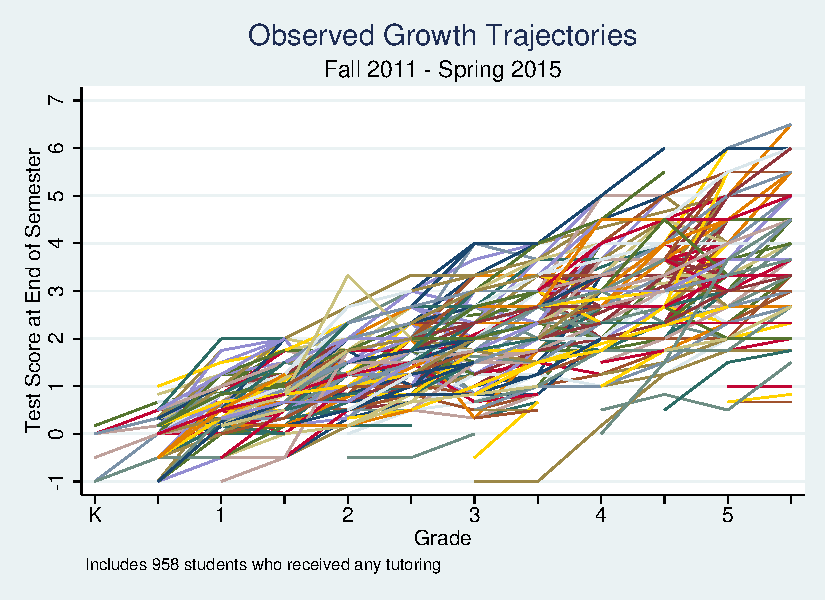
\includegraphics[width=0.8\linewidth]{xtline.pdf}
\captionof{figure}{\color{Green} Student Growth Trajectories}
\end{center}\vspace{1cm}

Explain graphic...

%----------------------------------------------------------------------------------------
%	CONCLUSIONS
%----------------------------------------------------------------------------------------

\color{SaddleBrown} % SaddleBrown color for the conclusions to make them stand out

\section*{Conclusions and Further Considerations}

\begin{itemize}
\item Vestibulum sem ante, hendrerit a gravida ac, blandit quis magna.
\item Donec sem metus, facilisis at condimentum eget, vehicula ut massa. Morbi consequat, diam sed convallis tincidunt, arcu nunc.
\item Nunc at convallis urna. isus ante. Pellentesque condimentum dui. Etiam sagittis purus non tellus tempor volutpat. Donec et dui non massa tristique adipiscing.
\end{itemize}

\color{DarkSlateGray} % Set the color back to DarkSlateGray for the rest of the content

\begin{center}\vspace{1cm}

\includegraphics[width=0.8\linewidth]{placeholder}
\captionof{figure}{\color{Green} Causal DAG}
\end{center}\vspace{1cm}

%----------------------------------------------------------------------------------------
%	ACKNOWLEDGEMENTS
%----------------------------------------------------------------------------------------

\section*{Acknowledgements}

Yukie Toyama, for providing guidance about the BUILD study and her work with the data set.

%----------------------------------------------------------------------------------------

\end{multicols}
\end{document}